\needspace{15\baselineskip}% room for the wrapped icon (it cannot break across pages)
\subsection{Solid oxide fuel cell on gas (4,100~\$/kW; with carbon capture 4,740~\$/kW)}\label{sec:sofc}
\techicon{sofc}{A solid oxide fuel cell stack: ceramic cells between interconnects; gas and air in, exhaust out.}
A solid oxide fuel cell (SOFC; Figure~\ref{fig:icon-sofc}) turns natural gas into electricity electrochemically, at 59\,\% efficiency, and operates as baseload because it is not suited for ramping.
Its exhaust is mostly CO$_2$ and water, so capture needs no solvent and is cheaper than after a turbine.
Table~\ref{tab:costs} therefore carries the fuel cell without and with capture; only the latter fits a (near-)carbon-neutral system.


Without capture, the CAPEX of 4,100~\$/kW is Bloom Energy's average price per kW but includes a margin \citep{bloom10k}; the fitted product cost at today's 1.4~GW plus installation would be 2,495~\$/kW.

The additional cost for carbon capture have to be estimated.
We here infer them from hypothetical 650~MW plants built from SOFC stacks by NETL \citep{netl2022}.
There, capture adds 640~\$/kW (as the difference between a plant with and without CC 1,627 and 1,116~\$/kW) in 2018 dollars .
The value 640~\$/kW results from the economies of scale of a large 650 MW plant, and is likely less what CC would cost for a smaller Bloom plant.

The learning rate is 30\,\%, fitted to Bloom's product cost (Figure~\ref{fig:sofc}) and extrapolated to the CC component; it rests on one vendor's record and is high compared with similar technologies.
At this rate, the plant with capture reaches the cost of NETL's mature plant \citep{netl2022}, about 2,030~\$/kW in 2024 dollars, after about 2.4 doublings, near 7~GW of cumulative capacity.

\begin{figure}[htbp]\centering
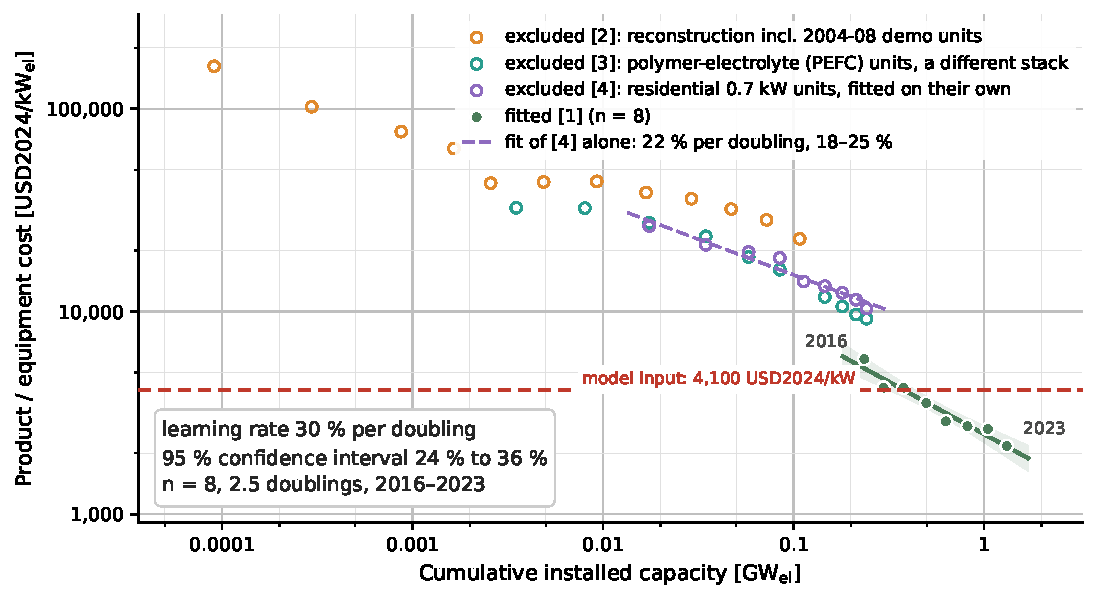
\includegraphics[width=\textwidth]{../../../misc-quarter1/technology-costs/figures/learning/sofc.pdf}
\caption{Fuel cell cost per kW against cumulative capacity.
Filled and fitted: Bloom Energy product cost [1] \citep{bloom10k}.
Hollow, for context: residential ENE-FARM units in Japan, as reconstructed by \citet{schmidt2018} [2] and from the official shipment statistics \citep{ace2025} for polymer-electrolyte [3] and solid oxide [4] units.
Dashed red line: the model input.}\label{fig:sofc}
\end{figure}

The fixed O\&M is 5\,\% of CAPEX per year, the DEA's figure for fuel cells \citep{dea}.
Capture lowers the efficiency to 0.55, removes 97.8\,\% of the CO$_2$ \citep{netl2022}.
We further assume this adds 4.5~\$/MWh for CO$_2$ transport and storage at NETL's 10~\$/t .
Existing capacity approximates Bloom's cumulative deployment, with no pipeline.
The lead time is 1~year \citep{eia2023}.

The gas price is the default of 20~\$/MWh\textsubscript{th} (Section~\ref{sec:CCGT}); where imported LNG sets the price, as in Europe, the model should add the cost of liquefaction.

The stacks last about five years and must be replaced, which the cost assumptions do not yet reflect.
